
\lecture{Introduction}{Introduction}
\section{Introduction}

\title{Statistics}
\subtitle{Introduction To Statistics and Course Information}

%\author{Kelly Black}
%\institute{Clarkson University}
\date{9 January 2015}

\begin{frame}
  \titlepage
\end{frame}

\begin{frame}
  \frametitle{Outline}
  \tableofcontents[hideothersubsections,sectionstyle=show/hide]
\end{frame}


\subsection{Class Information}


\begin{frame}
  \frametitle{Class Information}

\begin{description}
\item[Textbook] {\em Fundamentals of Statistics}, Third Edition, by
  Michael Sullivan, III, Prentice Hall;. (ISBN 0-321-64187) The book
  is available at the bookstore as well as many on-line outlets.

\end{description}

\end{frame}


\begin{frame}
  \frametitle{Class Information}

\begin{description}
\item[Grading] %~ \\ %\samepage
  
  The final grades are calculated using the following distribution:
    \begin{tabular}[t]{rl}
      60\% & Three Exams, \\
      17\% & Quizzes, \\
      17\% & Webworks, \\
      6\%  & Attendance/Clicker Response \\
    \end{tabular}
  
    At the end of the semester we assign letter grades as follows:
    97\% for an A+, 93\% for an A, 90\% for an A-, 
    87\% for a  B+, 83\% for an B, 80\% for a B-, 
    77\% for a  C+, 73\% for an C, 70\% for a C-, 
    and \%60 for a D.

\end{description}

\end{frame}



\begin{frame}
  \frametitle{Class Information}

\begin{description}
\item[Exam Dates] The first test is tentatively scheduled for Tuesday,
  10 February 2015, at 07:00 PM in Science Center 360. The second test
  is tentatively scheduled for Thursday, 12 March 2015, at 07:00 PM in
  Science Center 360 . The third test will take place during finals
  week at the time scheduled for the final exam. (There will not be a
  final exam.) You should bring your own pencils, blank paper,
  calculators, and good luck charms.  The professor will not have any
  spare materials.
 
\end{description}

\end{frame}

\begin{frame}
  \frametitle{Class Information}

\begin{description}
\item[Quiz] There will be a quizzes most weeks in your recitation. The
  quizzes will be similar to the posted homework problems. There will
  additional quizzes during lecture. Some will be announced in
  advance, and there will be unannounced quizzes during the lecture
  sessions.  Your lowest quiz score will be dropped.

\end{description}

\end{frame}


\begin{frame}
  \frametitle{Class Information}

\begin{description}
  \item[Clickers] A portion of your grade is for classroom attendance
    and participation. This is measured using clickers. Each day one
    or more questions will be asked, and you will be asked to respond
    using the clicker. The clicker that we are using is from Turning
    Point Technologies, and we recommend that you use the ResponseCard
    RF LCD clicker. You can purchase the clicker at
    \url{https://store.turningtechnologies.com} The Clarkson
    University promotional code is Z0k0.

\end{description}

\end{frame}

\begin{frame}
  \frametitle{Clickers}

  We will start using the clickers Friday, 16 January 2015. Each day
  one or more questions will be asked.

  You need to register your clicker. You should have received an email
  with instructions on how to do this. 

  \textbf{Note: Zero is not an ``O''  !!!}
  
\end{frame}


\begin{frame}
  \frametitle{Class Information}

\begin{description}
  \item[Webwork] Webwork is a web based homework system. You can find
    it at the following URL: \\
    \url{http://black.sc.clarkson.edu/webwork2/}.
\end{description}

\end{frame}


\begin{frame}
  \frametitle{Class Information}

\begin{description}
  \item[Academic Accommodations] If you require any kind of special
    accommodation please come see me.  Requests for academic
    accommodations must be made during the first three weeks of the
    semester, except for unusual circumstances.  Students must
    register with the Office of Accommodative Services, located in the
    Student Success Center, 110 ERC, to verify their eligibility for
    appropriate accommodations.


\end{description}


\end{frame}

\begin{frame}
  \frametitle{Class Information}

\begin{description}
\item[Office Hours] My office hours are from 9am to 10:30am on
  Mondays, Wednesdays, and Fridays. There are additional office hours
  from 10am to 11:30am on Tuesdays. Please contact Prof. Black to
  schedule other times to meet.

\end{description}


\end{frame}

\subsection{Data (Fukushima Radiation Survey)}

\begin{frame}
  \frametitle{Data}

  Different kinds of data....

  \uncover<2>{Be careful how to interpret data!}

\end{frame}

\begin{frame}
  \frametitle{Example Data Set}

  Fukushima Radiation Survey

  Measurements taken during the 11 march 2011 crisis after the
  T\={o}hoku earthquake:
  \begin{itemize}
  \item Time
  \item Date
  \item Longitude
  \item Latitude
  \item Distance From Source
  \item Direction From Source
  \item Radiation Level (mRad/hour)
  \item Description
  \item several others
  \end{itemize}

\end{frame}



\begin{frame}
  \frametitle{Direction}

  \begin{tabular}{c}
    Direction \\ \hline 
    N   \\
    NNE  \\
    NNW  \\
    NW  \\
    S  \\
    SSW \\
    SW  \\
    W  \\
    WNW  \\
    WSW 
  \end{tabular}

\end{frame}

\begin{frame}
  \frametitle{Direction}

  \begin{tabular}{c|c}
    Direction & Number \\ \hline
    N  & 7 \\
    NNE & 6 \\
    NNW & 21 \\
    NW   & 45 \\
    S  & 13 \\
    SSW  & 484 \\
    SW   & 958 \\
    W & 118 \\
    WNW & 32 \\
    WSW & 218
  \end{tabular}

\end{frame}

\subsection{Graphical View of Data}

\begin{frame}
  \frametitle{Direction - Bar Chart}

  \begin{center}
    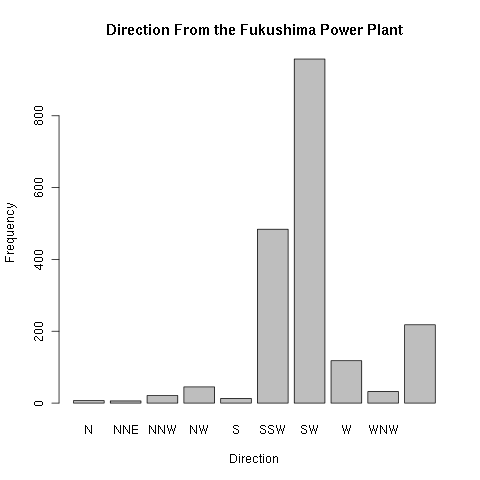
\includegraphics[width=8cm]{img/fukushimaDirectionBarPlot}
  \end{center}

\end{frame}

\begin{frame}
  \frametitle{Direction - Pareto Chart}

  \begin{center}
    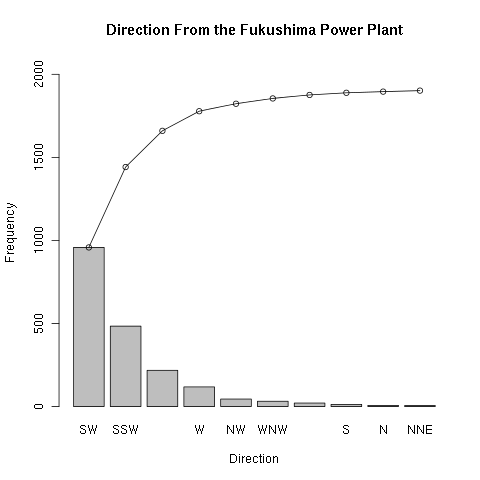
\includegraphics[width=8cm]{img/fukushimaParetoDirection}
  \end{center}

\end{frame}

\begin{frame}
  \frametitle{Radiation Data}

  \begin{center}
    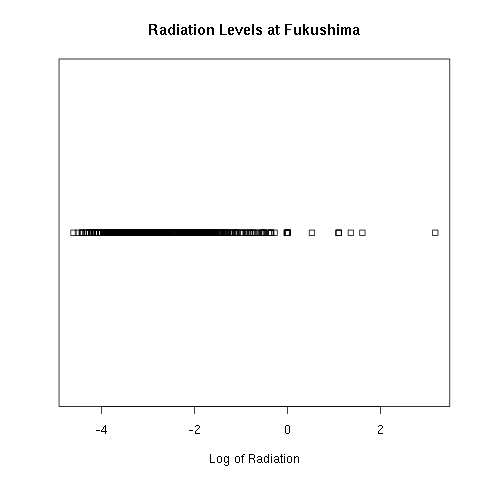
\includegraphics[width=8cm]{img/logFukushimaGamma}
  \end{center}  

\end{frame}

\begin{frame}
  \frametitle{Radiation Data}

  \begin{center}
    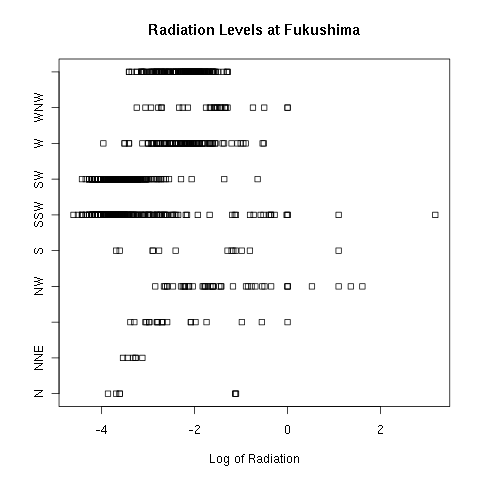
\includegraphics[width=8cm]{img/logFukushimaGammaByDirection}
  \end{center}  

\end{frame}


\begin{frame}{Why is the data spread out?}

  Problem: The data has a random component. Different measurements at
  different times give different radiation levels. 

  \vfill

  There is spread in the data and there are probabilities associated
  with how likely you are to get a certain range of measurements.

  \vfill
  
\end{frame}

\begin{frame}{Probability}

  What is probability?

  \begin{definition}[Probability]
    ``\textbf{Probability} is the measure of the likelihood of a random
    phenomena or chance behavior. Probability describes the long-term
    proportion with which a certain \textbf{outcome} will occur in
    situations with short-term uncertainty.'' (Page 223)
  \end{definition}

  
\end{frame}

\begin{frame}{Example}

  Everybody flip a coin once.

  \uncover<2->%
  {

    What did you get?

  }

  \uncover<3->%
  {

    Do it again!

  }

  \uncover<4->%
  {

    What did you get?

  }

  \uncover<5->%
  {

    Do it again!

  }

  \uncover<6->%
  {

    What did you get?

  }


  \uncover<7->%
  {

    (Four people) Flip a coin

  }

  \uncover<8->%
  {

    What did you get?

  }

  
\end{frame}

\begin{frame}{What the heck are we doing?}

  \begin{description}
  \item[Event:] Something that \textit{can} happen.
  \item[Outcome:] Something that did happen.
  \item[Experiment:] A structured activity that includes the
    measurement of the outcomes of the activity after predefined and
    intentional changes to some aspect of the events.
  \item[Observational Study:] A structured activity that includes the
    measurement of the outcomes of the activity without intentional
    changes to the events.
  \item[Expected Outcome:] The ``average'' of the possible outcomes.
  \item[Variation:] Some measure of the spread of possible outcomes.
  \end{description}
  
\end{frame}

\begin{frame}{Probability vs. Statistics}

  ``Probability'' is an idealized notion. If we repeat the experiment
  an infinite number of times we ask what \textit{will} happen.

  \vfill

  ``Statistics'' is the study of how to interpret data. We ask what
  ``did'' happen and what does it imply about the underlying
  probabilities?

  \vfill

  \uncover<2->%
  {

    Problem: We need to have a basic understanding of probability
    before we can do statistics.

  }
  
\end{frame}

% LocalWords:  Clarkson pausesection hideallsubsections Cuby Webworks Webwork
% LocalWords:  ResponseCard Fukushima hideothersubsections sectionstyle
